\documentclass[11pt, a4paper]{article}

\usepackage[a4paper, margin=2.5cm, top=2.5cm, bottom=2.5cm]{geometry}
\usepackage[UTF8,fontset=mac]{ctex}
\usepackage{fontspec}
\usepackage{amsmath, amssymb, amsthm}
\usepackage{booktabs}
\usepackage{tabularx}
\usepackage{fancyhdr}
\usepackage{enumitem}
\usepackage{xcolor}
\usepackage[unicode, bookmarksnumbered=true]{hyperref}
\usepackage{CJKfntef}
\usepackage{printlen} % 引入打印长度的宏包
\usepackage{array}
\usepackage{listings}    % 代码块支持
\usepackage{titlesec}
\usepackage{graphicx}     % 图片导入
\usepackage{float}        % 动态格式
\usepackage{multirow}
\usepackage{fontspec}

% 字体
\setmonofont{Fira Mono}
\setCJKmainfont[
    UprightFont = {Songti SC Light},
    BoldFont = {Heiti SC Medium}
]{Songti SC}
\newcommand{\heitiBold}[1]{%
    \raisebox{-0.04em}{\textbf{#1}}%
}
\newcommand{\Bunderdot}[1]{% 加粗 + 下加点
    \CJKunderdot{\raisebox{-0.04em}{\textbf{#1}}}
}
\newCJKfontfamily{\kaiti}{Kaiti SC}

% 一级标题：居中、大号、加粗
\titleformat{\section}
    {\centering\Large\bfseries}
    {\thesection}
    {1em}
    {}
% 二级标题：左对齐、较大、加粗
\titleformat{\subsection}
    {\large\bfseries}
    {}
    {0pt}
    {【}
    [】]

% 页眉页脚设置
\pagestyle{fancy}
\fancyhf{}
\newcommand{\currentproblem}{}% 当前题目的中文名称
\fancyhead[L]{\small 2026 CCF 非专业级软件能力认证 CSP-J/S 2026 第二轮} % 左上角：考试名称
\fancyhead[R]{\small 入门组\ \currentproblem} % 右上角：组别 + 当前题目名称
\fancyfoot[C]{%
    \small 第 \thepage\ 页 \hspace{1em} 共 \textcolor{blue}{\pdfpagerefbox} 页
} % 页脚：总页数用蓝色显示
\renewcommand{\headrulewidth}{0.4pt}
\renewcommand{\footrulewidth}{0pt}
\newcommand{\pdfpagerefbox}{12} % 手动设置总页数

% 首页专用页眉页脚样式
\fancypagestyle{firstpage}{
    \fancyhf{}
    \renewcommand{\headrulewidth}{0pt}
}

% 自定义环境与命令
% 每道题作为一级 section
\newcommand{\problemheading}[2]{%
    \clearpage
    \pdfbookmark[0]{#1（#2）}{#2}%
    \renewcommand{\currentproblem}{#1（#2）}%
    \section*{#1 (#2)}%
}
% 题目内部标题作为二级 subsection
\newcommand{\sectionbox}[2]{
    \vspace{1.3em}%
    \noindent\hspace*{1em}%
    \pdfbookmark[1]{#1}{#2}%
    {\large\bfseries【#1】}\par
    \vspace{0.4em}%
}
% 第一个题目内部标题
\newcommand{\sectionboxfirst}[2]{%
    \noindent\hspace*{1em}%
    \pdfbookmark[1]{#1}{#2}%
    {\large\bfseries【#1】}\par
    \vspace{0.4em}%
}

% 配置代码块样式 (Consolas字体, 行号, 语法高亮)
\lstset{
    basicstyle=\ttfamily\small,
    frame=single,
    rulecolor=\color{blue},
    framerule=0.4pt,
    breaklines=true,
    keywordstyle=\color{blue},
    commentstyle=\color{green!60!black},
    stringstyle=\color{red},
    numbers=left,
    numberstyle=\footnotesize\color{gray}\texttt,
    numbersep=8pt,
    xleftmargin=1.5em,
    framexleftmargin=0pt,
    tabsize=4,
    columns=fixed,
    keepspaces=true
}

% 缩短枚举元素间距离
\setlist[itemize]{
    itemsep=0pt,
    parsep=0pt,
    topsep=2pt,
    partopsep=0pt
}
\setlist[enumerate]{
    itemsep=0pt,
    parsep=0pt,
    topsep=2pt,
    partopsep=0pt
}

\xeCJKsetup{
  underdot/boxdepth = 0pt
}

\setlength{\intextsep}{0pt}

\begin{document}

% ------------------ Page 1: 首页须知 ------------------
\thispagestyle{firstpage}

\begin{center}
    {\Huge \heitiBold{2026 CCF 非专业级软件能力认证}}\\[1.5em]
    {\Huge CSP-J/S 2026 \heitiBold{第二轮}}\\[1em]
    {\Huge\kaiti 入门组}\\[0.5em]
    {\Large 时间: 2026年10月31日 08:30 $\sim$ 12:00}
\end{center}

\vspace{1em}

\noindent
\begin{tabular}{|p{3cm}|p{2.7cm}|p{2.7cm}|p{2.7cm}|p{2.7cm}|}
    \hline
    题目名称 & 旅游 & 回文串 & 按位与 & 纸牌游戏 \\ \hline
    题目类型 & 传统型 & 传统型 & 传统型 & 传统型 \\ \hline
    目录 & \texttt{travel} & \texttt{string} & \texttt{and} & \texttt{card} \\ \hline
    可执行文件名 & \texttt{travel} & \texttt{string} & \texttt{and} & \texttt{card} \\ \hline
    输入文件名 & \texttt{travel.in} & \texttt{string.in} & \texttt{and.in} & \texttt{card.in} \\ \hline
    输出文件名 & \texttt{travel.out} & \texttt{string.out} & \texttt{and.out} & \texttt{card.out} \\ \hline
    每个测试点时限 & 1.0秒 & 1.0秒 & 1.0秒 & 1.0秒 \\ \hline
    内存限制 & 1024 MiB & 1024 MiB & 1024 MiB & 1024 MiB \\ \hline
    测试点数目 & 20 & 25 & 20 & 25 \\ \hline
    测试点是否等分 & 是 & 是 & 是 & 是 \\ \hline
\end{tabular}

\vspace{1em}

提交源程序文件名

\vspace{0.5em}

\noindent
\begin{tabular}{|p{3cm}|p{2.7cm}|p{2.7cm}|p{2.7cm}|p{2.7cm}|}
    \hline
    对于 \texttt{C++} 语言 & \texttt{travel.cpp} & \texttt{string.cpp} & \texttt{and.cpp} & \texttt{card.cpp} \\ \hline
\end{tabular}

\vspace{0.5em}

编译选项

\vspace{0.5em}

\noindent
\begin{tabular}{|p{3.0cm}|>{\centering\arraybackslash}p{12.1cm}|}
    \hline
    对于 \texttt{C++} 语言 & \texttt{-O2 -std=c++14 -static} \\ \hline
\end{tabular}

\vspace{1em}

\Bunderdot{注意事项（请仔细阅读）}
\begin{enumerate}[label=\arabic*., itemsep=2pt, topsep=4pt]
    \item 文件名（程序名和输入输出文件名）必须使用英文小写。
    \item \texttt{main()} 函数的返回值类型必须是 \texttt{int}，程序正常结束时的返回值必须是 0。
    \item 若无特殊说明，结果的比较方式为全文比较（过滤行末空格及文末换行）。
    \item 选手提交的程序源文件大小不得超过 100KiB。
    \item 程序可使用的栈空间内存限制与题目的内存限制一致。
    \item 禁止在提交的程序源文件中改变编译器参数（如使用 \texttt{\#pragma} 命令），禁止使用系统结构相关指令（如内联汇编）或其他可能造成不公平的方法。
    \item 提交的程序源文件的放置位置请参考各省的具体要求。
    \item 因违反上述规定而出现的问题，申诉时一律不予受理。
    \item 只提供 Linux 格式附加样例文件。
    \item 全国统一评测时采用的机器配置为：Intel Core Ultra 9 285K CPU @ 3.70 GHz（关闭睿频与能效核），内存 96 GB。上述时限以此配置为准。
    \item 评测在当前最新公布的 NOI Linux 下进行，各语言的编译器版本以此为准。
\end{enumerate}

% ------------------ Page 2: 旅游（travel） ------------------

\problemheading{旅游}{travel}

\sectionboxfirst{题目描述}{T1-1}

小 R 和小 X 准备坐高铁出门旅游。他们买了两张二等座车票，车票上写着各自的车厢号和座位号。两人希望座位相邻，这样旅途中可以坐在一起。

他们乘坐的列车由 $17$ 节车厢组成，车厢编号是 \texttt{01} 到 \texttt{17}。其中，\texttt{01} 和 \texttt{16} 号车厢是一等座车厢，其余车厢是二等座车厢。两人买的都是二等座车票，座位都在二等座车厢中。每节二等座车厢共有 $18$ 排，每排有 $5$ 个座位。座位号由两位排号和一位大写字母组成，例如 \texttt{03C} 表示第 $3$ 排 C 座。每一排的座位按照从左到右的顺序排列，座位字母依次是 \texttt{A}、\texttt{B}、\texttt{C}、\texttt{D}、\texttt{F}，其中 C 座与 D 座之间是过道，即每排过道左侧的座位序列是 \texttt{A}、\texttt{B}、\texttt{C}，右侧是 \texttt{D}、\texttt{F}。以下是一节二等座车厢的座位示意图：

\vspace{0.3em}

\begin{figure}[H]
    \centering
    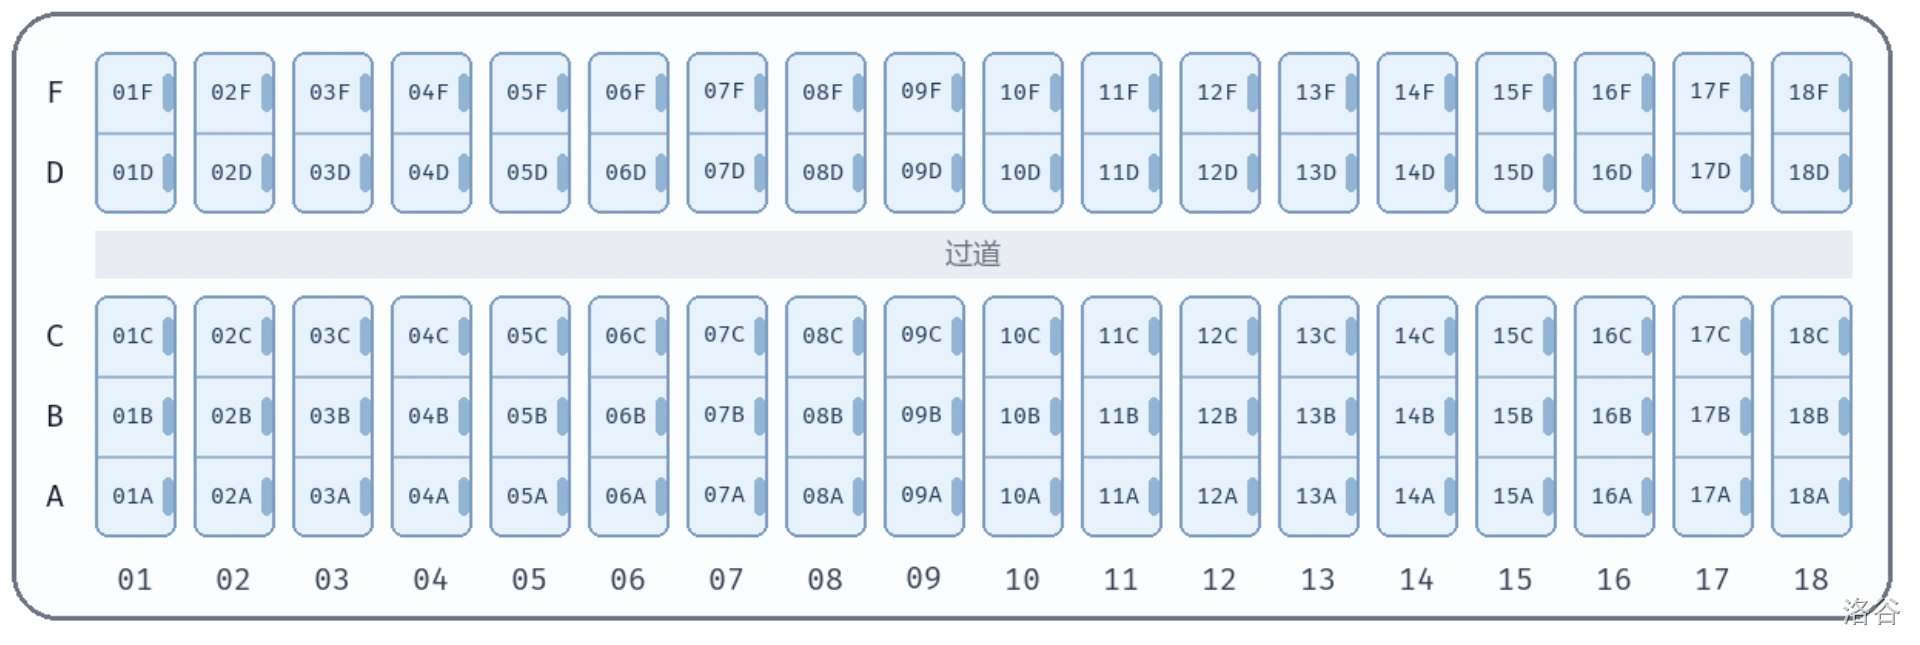
\includegraphics[width=1\textwidth]{hj5s80cz.png}
    \label{fig:T1}
\end{figure}

两个座位相邻，当且仅当在同一节车厢的同一排，位于过道的同一侧，且在该侧的座位序列中相邻。

你需要帮助小 R 依次判断：
\begin{itemize}
    \item 两张车票对应的座位是否在同一节车厢；
    \item 两张车票对应的座位是否在同一节车厢的同一排；
    \item 两张车票对应的座位是否在同一节车厢的同一排，且位于过道的同一侧；
    \item 两张车票对应的座位是否相邻。
\end{itemize}

\sectionbox{输入格式}{T1-2}

从文件 $\boldsymbol{travel.in}$ 中读入数据。

输入的第一行包含四个字符串 $c_1,s_1,c_2,s_2$，分别表示小 R 的车票上的车厢号、座位号，以及小 X 的车票上的车厢号、座位号。

\sectionbox{输出格式}{T1-3}

输出到文件 $\boldsymbol{travel.out}$ 中。

输出一行一个长度为 $4$ 的 \texttt{01} 字符串，分别表示四个问题的答案，其中 \texttt{1} 代表是，\texttt{0} 代表否。

\clearpage % ！！！找到合适尺寸后移除

\sectionbox{样例1输入}{T1-4}
\begin{lstlisting}
02 01A 02 01B
\end{lstlisting}

\sectionbox{样例1输出}{T1-5}
\begin{lstlisting}
1111
\end{lstlisting}

\sectionbox{样例1解释}{T1-6}
\texttt{02} 号车厢是二等座车厢。\texttt{01A} 和 \texttt{01B} 在同一节车厢、同一排、过道的同一侧，并且相邻，因此输出 \texttt{1111}。

\sectionbox{样例2输入}{T1-7}
\begin{lstlisting}
02 01C 02 01A
\end{lstlisting}

\sectionbox{样例2输出}{T1-8}
\begin{lstlisting}
1110
\end{lstlisting}

\sectionbox{样例2解释}{T1-9}
两个座位在同一节车厢、同一排、过道的同一侧，但 \texttt{01C} 与 \texttt{01A} 中间隔着 \texttt{01B}，不相邻，因此输出 \texttt{1110}。

\sectionbox{样例3输入}{T1-10}
\begin{lstlisting}
02 01C 02 01D
\end{lstlisting}

\sectionbox{样例3输出}{T1-11}
\begin{lstlisting}
1100
\end{lstlisting}

\sectionbox{样例4输入}{T1-12}
\begin{lstlisting}
02 02B 02 01A
\end{lstlisting}

\sectionbox{样例4输出}{T1-13}
\begin{lstlisting}
1000
\end{lstlisting}

\clearpage % ！！！找到合适尺寸后移除

\sectionbox{样例5输入}{T1-14}
\begin{lstlisting}
02 01A 03 01A
\end{lstlisting}

\sectionbox{样例5输出}{T1-15}
\begin{lstlisting}
0000
\end{lstlisting}

\sectionbox{数据范围}{T1-16}

对于所有测试数据，均有：
\begin{itemize}
    \item $c_1,c_2$ 是 \texttt{01} 到 \texttt{17} 之间除 \texttt{01} 和 \texttt{16} 外的两位车厢号；
    \item $s_1,s_2$ 是对应车厢中的合法座位号，即前两位是 \texttt{01} 到 \texttt{18} 之间的排号，末位是 \texttt{A}、\texttt{B}、\texttt{C}、\texttt{D}、\texttt{F} 中的一个字母；
    \item 两张车票对应的不是同一个座位，即 $c_1\ne c_2$ 或 $s_1\ne s_2$。
\end{itemize}

\begin{center}
\renewcommand{\arraystretch}{1}
\setlength{\arrayrulewidth}{0.5pt}
\begin{tabular}{c!{\vrule width 0.6pt}c}
    \noalign{\hrule height 1.5pt}
    测试点编号 & 特殊性质 \\
    \noalign{\hrule height 1pt}
    1 $\sim$ 4   & A、B、C \\
    \hline
    5 $\sim$ 10  & A、B \\
    \hline
    11 $\sim$ 14 & A \\
    \hline
    15 $\sim$ 17 & D \\
    \hline
    18 $\sim$ 20 & 无 \\
    \noalign{\hrule height 1.5pt}
\end{tabular}
\end{center}

特殊性质 A：两个座位在同一节车厢，即 $c_1=c_2$。

特殊性质 B：两个座位在同一排，即 $s_1$ 的前两位与 $s_2$ 的前两位相同。

特殊性质 C：两个座位在过道的同一侧。

特殊性质 D：小 R 的座位是 D 座，小 X 的座位是 F 座，即 $s_1$ 的末位字符是 \texttt{D}，$s_2$ 的末位字符是 \texttt{F}。

% ------------------ Page 5: 回文串（string） ------------------

\problemheading{回文串}{string}

\sectionboxfirst{题目描述}{T2-1}

小 R 有一个长度为 $L$ 的字符串 $S=s_1\ldots s_L$，其中只包含小写英文字母。小 R 发现，虽然 $S$ 可能很长，但它可以分成 $n$ 个连续的段，其中第 $i\ (1\le i\le n)$ 段由 $a_i$ 个小写英文字母 $c_i$ 构成。把这 $n$ 段依次拼接起来便得到 $S$，因此 $L=\sum_{i=1}^{n}a_i$。相邻两段中的字符可以相同。

小 X 喜欢回文串。若一个字符串反转后与原字符串相同，就称它是回文串，例如 \texttt{aba}、\texttt{abba} 都是回文串，而 \texttt{aabbc} 不是。也就是说，字符串 $S$ 是回文串，当且仅当对于所有 $i\ (1\le i\le L)$，均有 $s_i=s_{L+1-i}$。

小 X 想让小 R 把 $S$ 改成回文串。小 R 可以将 $S$ 中任意一个位置的字符修改成任意小写英文字母。他想用尽量少的修改满足小 X 的要求。

你需要帮助小 R 求出，他最少需要修改多少个位置的字符，才能将 $S$ 改成回文串。

\sectionbox{输入格式}{T2-2}

从文件 $\boldsymbol{string.in}$ 中读入数据。

输入的第一行包含一个正整数 $n$。

输入的第 $i+1\ (1\le i\le n)$ 行包含一个正整数 $a_i$ 和一个小写英文字母 $c_i$。

\sectionbox{输出格式}{T2-3}

输出到文件 $\boldsymbol{string.out}$ 中。

输出一行一个整数，表示小 R 最少需要修改多少个位置的字符，才能将 $S$ 改成回文串。

\sectionbox{样例1输入}{T2-4}
\begin{lstlisting}
3
2 a
2 b
1 c
\end{lstlisting}

\sectionbox{样例1输出}{T2-5}
\begin{lstlisting}
2
\end{lstlisting}

\sectionbox{样例1解释}{T2-6}

小 R 的字符串 $S$ 由 $3$ 段构成：第 $1$ 段由 $2$ 个 \texttt{a} 组成，第 $2$ 段由 $2$ 个 \texttt{b} 组成，第 $3$ 段由 $1$ 个 \texttt{c} 组成，依次拼接得到 $S=\mathtt{aabbc}$。

小 R 可以将最后一个字符 \texttt{c} 和倒数第二个字符 \texttt{b} 都改为 \texttt{a}，得到回文串 \texttt{aabaa}，共修改 $2$ 个位置的字符。可以证明，小 R 最少需要修改 $2$ 个位置的字符，才能将 $S$ 改成回文串。

\clearpage % ！！！找到合适尺寸后移除

\sectionbox{样例2输入}{T2-7}
\begin{lstlisting}
2
2 a
3 a
\end{lstlisting}

\sectionbox{样例2输出}{T2-8}
\begin{lstlisting}
0
\end{lstlisting}

\sectionbox{样例2解释}{T2-9}

小 R 的字符串 $S$ 由 $2$ 段构成：第 $1$ 段由 $2$ 个 \texttt{a} 组成，第 $2$ 段由 $3$ 个 \texttt{a} 组成，依次拼接得到 $S=\mathtt{aaaaa}$，则 $S$ 已经是回文串，不需要修改。

\sectionbox{样例3输入}{T2-10}
\begin{lstlisting}
6
1000000000 a
1000000000 a
1000000000 a
1000000000 b
1000000000 b
1000000000 b
\end{lstlisting}

\sectionbox{样例3输出}{T2-11}
\begin{lstlisting}
3000000000
\end{lstlisting}

\sectionbox{样例4}{T2-12}
见题目目录下的 $\boldsymbol{string/4.in}$ 与 $\boldsymbol{string/4.ans}$。

该样例满足测试点 $10\sim 12$ 的约束条件。

\sectionbox{样例5}{T2-13}
见题目目录下的 $\boldsymbol{string/5.in}$ 与 $\boldsymbol{string/5.ans}$。

该样例满足测试点 $13\sim 16$ 的约束条件。

\sectionbox{样例6}{T2-14}
见题目目录下的 $\boldsymbol{string/6.in}$ 与 $\boldsymbol{string/6.ans}$。

该样例满足测试点 $19\sim 21$ 的约束条件。

\clearpage % ！！！找到合适尺寸后移除

\sectionbox{数据范围}{T2-15}

对于所有测试数据，均有：

\begin{itemize}
    \item $1\le n\le 2\times10^5$；
    \item 对于所有 $i\ (1\le i\le n)$，均有 $1\le a_i\le10^9$，且 $c_i$ 为小写英文字母。
\end{itemize}

\vspace{0.5em}
\noindent
\begin{center}
\renewcommand{\arraystretch}{1}
\setlength{\arrayrulewidth}{0.5pt}
\begin{tabular}{c!{\vrule width 0.6pt}c!{\vrule width 0.6pt}c}
    \noalign{\hrule height 1.5pt}
    测试点编号 & $n\le$ & $\max_{i=1}^{n} a_i\le$ \\
    \noalign{\hrule height 1pt}

    1 & 1 & \multirow{2}{*}{5} \\
    \cline{1-2}
    2 $\sim$ 4 & 2 & \\

    \cline{1-3}
    5, 6 & \multirow{2}{*}{10} & 1 \\
    \cline{1-1}\cline{3-3}
    7, 8 & & 50 \\
    
    \cline{1-3}
    9 & \multirow{3}{*}{2000} & 1 \\
    \cline{1-1}\cline{3-3}
    10 $\sim$ 12 & & 50 \\
    \cline{1-1}\cline{3-3}
    13 $\sim$ 16 & & $10^9$ \\
    
    \cline{1-3}
    17, 18 & \multirow{3}{*}{$2\times10^5$} & 1 \\
    \cline{1-1}\cline{3-3}
    19 $\sim$ 21 & & 500 \\
    \cline{1-1}\cline{3-3}
    22 $\sim$ 25 & & $10^9$ \\

    \noalign{\hrule height 1.5pt}
\end{tabular}
\end{center}

% ------------------ Page 8: 按位与（and） ------------------

\problemheading{按位与}{and}

\sectionboxfirst{题目描述}{T3-1}

小 R 有 $n$ 个非负整数 $a_1,a_2,\ldots,a_n$。

小 X 给了小 R 一个正整数 $m$，并要求小 R 从这 $n$ 个非负整数中选出\Bunderdot{恰好}\, $m$ 个，使得选出的 $m$ 个数的\Bunderdot{二进制按位与}的值最大。

你需要帮助小 R 求出，他能选出的 $m$ 个数的按位与的最大值。

\sectionbox{输入格式}{T3-2}

从文件 $\boldsymbol{and.in}$ 中读入数据。

输入的第一行包含两个正整数 $n,m$。

输入的第二行包含 $n$ 个非负整数 $a_1,a_2,\ldots,a_n$，依次表示小 R 的 $n$ 个非负整数。

\sectionbox{输出格式}{T3-3}

输出到文件 $\boldsymbol{and.out}$ 中。

输出一行一个非负整数，表示小 R 能选出的 $m$ 个数的按位与的最大值。

\sectionbox{样例1输入}{T3-4}
\begin{lstlisting}
4 2
3 15 12 12
\end{lstlisting}

\sectionbox{样例1输出}{T3-5}
\begin{lstlisting}
12
\end{lstlisting}

\sectionbox{样例1解释}{T3-6}

小 R 有 $4$ 个非负整数：$3,15,12,12$。

\begin{itemize}
    \item 若小 R 选择 $3,15$，则按位与的值为 $3\mathbin{\mathrm{and}}15=3$；
    \item 若小 R 选择 $3,12$，则按位与的值为 $3\mathbin{\mathrm{and}}12=0$；
    \item 若小 R 选择 $15,12$，则按位与的值为 $15\mathbin{\mathrm{and}}12=12$；
    \item 若小 R 选择 $12,12$，则按位与的值为 $12\mathbin{\mathrm{and}}12=12$。
\end{itemize}

因此，小 R 能选出的 $m$ 个数的按位与的最大值为 $12$。

\sectionbox{样例2输入}{T3-7}
\begin{lstlisting}
5 3
31 3 1 15 7
\end{lstlisting}

\clearpage % ！！！找到合适尺寸后移除

\sectionbox{样例2输出}{T3-8}
\begin{lstlisting}
7
\end{lstlisting}

\sectionbox{样例2解释}{T3-9}

若小 R 选择 $31,15,7$，则按位与的值为 $31\mathbin{\mathrm{and}}15\mathbin{\mathrm{and}}7=7$。可以证明，小 R 能选出的 $m$ 个数的按位与的最大值为 $7$。

\sectionbox{样例3}{T3-10}
见题目目录下的 $\boldsymbol{and/3.in}$ 与 $\boldsymbol{and/3.ans}$。

该样例满足测试点 $8\sim 10$ 的约束条件。

\sectionbox{样例4}{T3-11}
见题目目录下的 $\boldsymbol{and/4.in}$ 与 $\boldsymbol{and/4.ans}$。

该样例满足测试点 $14,15$ 的约束条件。

\sectionbox{样例5}{T3-12}
见题目目录下的 $\boldsymbol{and/5.in}$ 与 $\boldsymbol{and/5.ans}$。

该样例满足测试点 $18,19$ 的约束条件。

\sectionbox{数据范围}{T3-13}

对于所有测试数据，均有：

\begin{itemize}
    \item $1\le m\le n\le 2\times 10^5$；
    \item 对于所有 $i$（$1\le i\le n$），均有 $0\le a_i<2^{30}$。
\end{itemize}

\vspace{0.5em}
\noindent
\begin{center}
\renewcommand{\arraystretch}{1}
\setlength{\arrayrulewidth}{0.5pt}
\begin{tabular}{c!{\vrule width 0.6pt}c!{\vrule width 0.6pt}c!{\vrule width 0.6pt}c!{\vrule width 0.6pt}c}
    \noalign{\hrule height 1.5pt}
    测试点编号 & $n\le$ & $m$ & $\max_{i=1}^n a_i<$ & 特殊性质\\
    \noalign{\hrule height 1pt}

    $1\sim 5$ & 20 & $\le n$ & \multirow{7}{*}{$2^{20}$} & \multirow{5}{*}{无} \\
    \cline{1-3}
    6 & \multirow{3}{*}{2000} & $=1$ & & \\
    \cline{1-1}\cline{3-3}
    7 & & $=n$ & & \\
    \cline{1-1}\cline{3-3}
    $8\sim 10$ & & $=2$ & & \\
    \cline{1-3}
    $11,12$ & \multirow{6}{*}{$2\times 10^5$} & $=n-1$ & & \\
    \cline{1-1}\cline{3-3}\cline{5-5}
    $13$ & & \multirow{5}{*}{$\le n$} & & A \\
    \cline{1-1}\cline{5-5}
    $14,15$ & & & & B \\
    \cline{1-1}\cline{4-5}
    $16,17$ & & & $4$ & \multirow{3}{*}{无} \\
    \cline{1-1}\cline{4-4}
    $18,19$ & & & $2^{10}$ & \\
    \cline{1-1}\cline{4-4}
    $20$ & & & $2^{30}$ & \\

    \noalign{\hrule height 1.5pt}
\end{tabular}
\end{center}

特殊性质 A：对于所有 $i$（$1\le i\le n$），均存在非负整数 $k_i$ 满足 $a_i=2^{k_i}-1$。

特殊性质 B：存在非负整数 $k$ 满足 $n=2^k$，且对所有 $i$（$1\le i\le n$），均有 $a_i=i-1$。

% ------------------ Page 10: 纸牌游戏（card） ------------------

\problemheading{纸牌游戏}{card}

\sectionboxfirst{题目描述}{T4-1}

小 Z 正在玩一种单人纸牌游戏。

他有一叠特制的纸牌，共有 $n$ 张，从上到下的点数依次为 $a_1,a_2,\ldots,a_n$。每张牌的点数都是 $1$ 到 $m$ 之间的整数，且每种点数都出现至少一次。

小 Z 将进行 $n$ 局相互独立的游戏。每局开始前，他会将所有牌按原顺序放回牌堆，并清空桌面。在第 $i$（$1\le i\le n$）局中，他跳过前 $i-1$ 张牌，依次打出第 $i$ 张到第 $n$ 张牌，这些牌的点数依次为 $a_i,a_{i+1},\ldots,a_n$。

桌面上的牌始终从左到右排成一行。打出一张点数为 $k$ 的牌时：

\begin{itemize}
    \item 若桌面上没有点数为 $k$ 的牌，就将这张牌放在最右端；
    \item 否则，收走桌面上点数为 $k$ 的牌及其右侧的所有牌，再把这张牌放在最右端。被收走的牌在本局中不再使用。
\end{itemize}

由上述规则可知，任意时刻桌面上同一种点数的牌至多只有一张。

最后一张牌打出后，本局游戏结束。

例如，若桌面上从左到右的牌的点数依次为 $1,4,2$，则打出一张点数为 $3$ 的牌后，桌面上从左到右的牌的点数依次为 $1,4,2,3$。接着打出一张点数为 $4$ 的牌时，桌面上原来点数为 $4$ 的牌及其右侧的所有牌（点数依次为 $4,2,3$）被收走，再把新打出的 $4$ 放在最右端，此时桌面上从左到右的牌的点数依次为 $1,4$。

你需要帮助小 Z 依次求出，对于每个 $i=1,2,\ldots,m$，在所有 $n$ 局游戏中，有多少局结束时桌面上留有点数为 $i$ 的牌。

\sectionbox{输入格式}{T4-2}

从文件 $\boldsymbol{card.in}$ 中读入数据。

输入的第一行包含两个正整数 $n,m$，分别表示牌的数量和点数种类数。

输入的第二行包含 $n$ 个正整数 $a_1,a_2,\ldots,a_n$，依次表示小 Z 的牌从上到下的点数。

\sectionbox{输出格式}{T4-3}

输出到文件 $\boldsymbol{card.out}$ 中。

输出一行 $m$ 个非负整数，其中第 $i$（$1\le i\le m$）个整数表示在所有 $n$ 局游戏中，有多少局结束时桌面上留有点数为 $i$ 的牌。

\sectionbox{样例1输入}{T4-4}
\begin{lstlisting}
4 3
1 2 1 3
\end{lstlisting}

\sectionbox{样例1输出}{T4-5}
\begin{lstlisting}
3 1 4
\end{lstlisting}

\sectionbox{样例1解释}{T4-6}

对于第 $1$ 局游戏，小 Z 依次打出点数为 $1,2,1,3$ 的牌：

\begin{enumerate}
    \item 打出第 $1$ 张牌（点数为 $1$）后，桌面上只有一张点数为 $1$ 的牌；
    \item 打出第 $2$ 张牌（点数为 $2$）后，桌面上从左到右的牌的点数依次为 $1,2$；
    \item 打出第 $3$ 张牌（点数为 $1$）后，先收走桌面上点数为 $1,2$ 的两张牌，再放上新打出的 $1$，桌面上只有一张点数为 $1$ 的牌；
    \item 打出第 $4$ 张牌（点数为 $3$）后，桌面上从左到右的牌的点数依次为 $1,3$。
\end{enumerate}

因此第 $1$ 局游戏结束时，桌面上从左到右的牌的点数依次为 $1,3$。

对于第 $2$ 局游戏，小 Z 依次打出点数为 $2,1,3$ 的牌，结束时桌面上从左到右的牌的点数依次为 $2,1,3$。

对于第 $3$ 局游戏，小 Z 依次打出点数为 $1,3$ 的牌，结束时桌面上从左到右的牌的点数依次为 $1,3$。

对于第 $4$ 局游戏，小 Z 仅打出一张点数为 $3$ 的牌，结束时桌面上只有一张点数为 $3$ 的牌。

因此，在全部 $4$ 局游戏中：

\begin{itemize}
    \item 有 $3$ 局游戏结束时，桌面上留有点数为 $1$ 的牌，即第 $1,2,3$ 局；
    \item 有 $1$ 局游戏结束时，桌面上留有点数为 $2$ 的牌，即第 $2$ 局；
    \item 有 $4$ 局游戏结束时，桌面上留有点数为 $3$ 的牌，即全部 $4$ 局。
\end{itemize}

\sectionbox{样例2输入}{T4-7}
\begin{lstlisting}
10 3
3 1 2 1 3 2 3 1 2 1
\end{lstlisting}

\sectionbox{样例2输出}{T4-8}
\begin{lstlisting}
10 3 3
\end{lstlisting}

\sectionbox{样例3}{T4-9}
见题目目录下的 $\boldsymbol{card/3.in}$ 与 $\boldsymbol{card/3.ans}$。

该样例满足测试点 $4\sim 6$ 的约束条件。

\sectionbox{样例4}{T4-10}
见题目目录下的 $\boldsymbol{card/4.in}$ 与 $\boldsymbol{card/4.ans}$。

该样例满足测试点 $7\sim 9$ 的约束条件。

\sectionbox{样例5}{T4-11}
见题目目录下的 $\boldsymbol{card/5.in}$ 与 $\boldsymbol{card/5.ans}$。

该样例满足测试点 $15\sim 17$ 的约束条件。

\clearpage % ！！！找到合适尺寸后移除

\sectionbox{样例6}{T4-12}
见题目目录下的 $\boldsymbol{card/6.in}$ 与 $\boldsymbol{card/6.ans}$。

该样例满足测试点 $21,22$ 的约束条件。

\sectionbox{数据范围}{T4-13}

对于所有测试数据，均有：

\begin{itemize}
    \item $2\le n\le 5\times 10^5$，$1\le m\le 3\times 10^5$；
    \item 对于所有 $i$（$1\le i\le n$），均有 $1\le a_i\le m$；
    \item 每种点数都出现至少一次，即对于所有 $i$（$1\le i\le m$），均存在 $j$（$1\le j\le n$）满足 $a_j=i$。
\end{itemize}

\vspace{0.5em}
\noindent
\begin{center}
\renewcommand{\arraystretch}{1}
\setlength{\arrayrulewidth}{0.5pt}
\begin{tabular}{c!{\vrule width 0.6pt}c!{\vrule width 0.6pt}c!{\vrule width 0.6pt}c}
    \noalign{\hrule height 1.5pt}
    测试点编号 & $n\le$ & $m\le$ & 特殊性质\\
    \noalign{\hrule height 1pt}

    $1\sim 3$ & 5 & 2 & \multirow{2}{*}{无} \\
    \cline{1-3}
    $4\sim 6$ & 500 & 200 & \\
    \cline{1-4}
    $7\sim 9$ & \multirow{2}{*}{5000} & \multirow{2}{*}{3000} & A \\
    \cline{1-1}\cline{4-4}
    $10\sim 12$ & & & \multirow{2}{*}{无} \\
    \cline{1-3}
    $13,14$ & \multirow{5}{*}{$2\times 10^5$} & 2 & \\
    \cline{1-1}\cline{3-4}
    $15\sim 17$ & & \multirow{2}{*}{3000} & B \\
    \cline{1-1}\cline{4-4}
    $18,19$ & & & 无 \\
    \cline{1-1}\cline{3-4}
    $20$ & & \multirow{2}{*}{$10^5$} & A \\
    \cline{1-1}\cline{4-4}
    $21,22$ & & & \multirow{2}{*}{无} \\
    \cline{1-3}
    $23\sim 25$ & $5\times 10^5$ & $3\times 10^5$ & \\

    \noalign{\hrule height 1.5pt}  %11
\end{tabular}
\end{center}

特殊性质 A：$a_1\le a_2\le\cdots\le a_n$。

特殊性质 B：至多存在 $4999$ 个 $i$（$1\le i\le n-1$）满足 $a_i\ne a_{i+1}$。

\end{document}